\documentclass[10pt,twocolumn,letterpaper]{article}

% ---------- Page layout (close to ICML / NeurIPS-style preprint) ----------
\usepackage[letterpaper,top=0.9in,bottom=1in,left=0.75in,right=0.75in,columnsep=0.25in]{geometry}
\usepackage[T1]{fontenc}
\usepackage{mathptmx}
\usepackage{microtype}
\usepackage{amsmath,amssymb}
\usepackage{booktabs}
\usepackage{multirow}
\usepackage{graphicx}
\usepackage{xcolor}
\usepackage{natbib}
\usepackage[font=small,labelfont=bf,skip=4pt]{caption}
\usepackage{enumitem}
\usepackage{titlesec}
\usepackage{tikz}
\usetikzlibrary{arrows.meta,positioning,fit,calc}
\usepackage{fancyhdr}
\usepackage[colorlinks=true,linkcolor=blue!50!black,citecolor=blue!50!black,urlcolor=blue!50!black]{hyperref}

\setcitestyle{authoryear,round,aysep={},yysep={,}}
\setlist{leftmargin=1.2em,itemsep=1pt,topsep=2pt,parsep=0pt}
\titleformat{\section}{\normalfont\large\bfseries}{\thesection}{0.6em}{}
\titleformat{\subsection}{\normalfont\normalsize\bfseries}{\thesubsection}{0.6em}{}
\titlespacing*{\section}{0pt}{9pt plus 2pt minus 2pt}{4pt}
\titlespacing*{\subsection}{0pt}{7pt plus 2pt minus 2pt}{3pt}
\setlength{\parskip}{0pt}
\titlespacing*{\paragraph}{0pt}{4pt plus 1pt minus 1pt}{0.6em}
\setlength{\textfloatsep}{10pt plus 2pt minus 2pt}

\newcommand{\todo}[1]{\textcolor{red!75!black}{[#1]}}
\newcommand{\ours}{\textsc{PathPlanner}}

\pagestyle{fancy}
\fancyhf{}
\renewcommand{\headrulewidth}{0pt}
\fancyhead[C]{\footnotesize\itshape Preprint. Draft of November 23, 2026.}
\fancyfoot[C]{\thepage}

% ------------------------------------------------------------------------
\begin{document}

\twocolumn[
\begin{center}
{\LARGE\bfseries Neural Transformer: Predicting a Token's\\[3pt]
Full Neuron Path Ahead of Time in SwiGLU Language Models\par}
\vspace{14pt}
{\large Travis Waters\par}
\vspace{2pt}
{\normalsize Independent Researcher\par}
\vspace{16pt}
\end{center}
]

\begin{abstract}
\noindent It is already known that LLMs do not need all of their MLP neurons for every token. The extent to which this is true, and our ability to predict it, is not yet clear. This paper introduces the Neural Transformer (NT): a small transformer model trained to predict which neurons each remaining layer of a SwiGLU model should keep active, before those layers run. On Mistral-7B, we found that after running two layers densely, the Neural Transformer was able to predict which neurons to use in the remaining 30 layers with only a 5.2\% perplexity increase relative to the dense model, while keeping 49\% of neurons. At about the same retention, two other ahead-of-time methods, GRIFFIN and NeuroPrefetcher, increase perplexity by 72\% and 228\% respectively. In a HellaSwag evaluation, keeping only 20\% of neurons, the Neural Transformer is able to match GRIFFIN with 48\% retention. Ablations show that end-to-end training cuts the perplexity cost of imitation-trained predictors by 6 to 7 times, that fixed neuron groups and clustered pattern vocabularies discard most per-token sparsity, and that layer-by-layer generation beats one-shot prediction in two training seeds. The Neural Transformer also performed better on Mistral-7B than on Qwen3-1.7B, suggesting that it could be even more successful on larger models; further testing with larger models will be necessary to confirm this. All quality results simulate skipping by masking; turning them into faster inference remains open.
\end{abstract}

\begin{center}\small Code, results and a script that checks every number in this paper:\\ \url{https://github.com/travishub09/Neural-Transformers}\end{center}


% ------------------------------------------------------------------------
\section{Introduction}

A decoder-only language model evaluates every MLP neuron for every token, yet for any single token most neurons contribute little to the output. This \emph{contextual sparsity} is well documented: Deja Vu trains per-layer predictors to choose active neurons and attention heads on the fly \citep{liu2023dejavu}, and systems such as PowerInfer and LLM in a Flash use predicted sparsity to keep only the needed weights in fast memory \citep{song2024powerinfer,alizadeh2024flash}. Two questions remain open for modern models. How many neurons can a token really do without? And how early can we tell which ones it will need?

Both questions are harder than they look. Modern models use gated activations such as SwiGLU \citep{shazeer2020glu}, which rarely produce exact zeros, so there is no obvious set of ``off'' neurons to predict. Activation-label predictors that worked on ReLU models lose accuracy, and several recent methods either restore ReLU through retraining \citep{mirzadeh2023relu,song2025prosparse} or skip MLP sparsity on SwiGLU models altogether \citep{shrestha2025polar}. Methods that do target SwiGLU models either decide after a layer's activations are computed \citep{lee2024cats,liu2025teal}, which says nothing about how early the choice could be made, or decide early with a coarse rule: one neuron set for a whole sequence \citep{dong2024griffin}, or a pattern chosen from a clustered vocabulary \citep{dhar2026neuroprefetcher}. We find that these coarse rules degrade sharply once skipping covers most layers and all three MLP projections.

We study \textbf{upfront path planning}: after a small dense prefix, predict for the current token a per-neuron mask for every remaining layer before any of those layers run. We call a token's masks for all sparse layers its \emph{path}. Our method, the \textbf{Neural Transformer} (NT), is a small causal transformer whose sequence positions are the base model's layers and whose outputs are neuron masks: a transformer over neurons (Figure~\ref{fig:overview}). Starting from a context vector built from the token's hidden state after layer~2 and the previous token's path, it generates each layer's mask conditioned on the masks it has already chosen, much as a language model generates a sentence. We train it end to end through the frozen base model with a distillation objective and a compute penalty, rather than imitating activation labels. The answer it gives to the two questions above is that, on Mistral-7B, about half of a token's MLP neurons can be dropped for a 5.2\% perplexity increase, and which half is largely decided after two layers.

\paragraph{Why ahead of time matters in practice.} At batch size one, generating a token is limited by memory bandwidth: every weight is read once per token. A 7B-parameter model needs about 14.5\,GB in 16-bit precision and a 70B model about 140\,GB, more than many laptop GPUs, phones or a single 80\,GB accelerator hold. Weights that do not fit must be streamed from CPU memory or flash, over links far slower than on-package memory: a PCIe~4.0 $\times$16 link carries at most about 32\,GB/s and a fast NVMe drive about 7\,GB/s, against 2--3\,TB/s for HBM, so streaming all of Mistral-7B's weights takes roughly half a second per token over PCIe and about two seconds from flash. The MLP blocks hold about 78\% of Mistral-7B's parameters, and at 31\% retention the Neural Transformer's masks exclude roughly half of the model's total weights. A plan for every remaining layer, available after layer~2, is what would let such transfers be scheduled, batched and overlapped with computation instead of waiting on each layer. This paper measures quality only: skipping is simulated by masking a dense computation, and turning the plan into faster decoding is systems work that we begin, but do not finish, in Section~\ref{sec:deploy}.

Our contributions are:
\begin{itemize}
\item \textbf{The Neural Transformer}, which predicts a token's full per-neuron MLP path after two dense layers, generated layer by layer, for frozen SwiGLU models. With the same inputs, layer-by-layer generation beats one-shot prediction by 3.4 to 6.5 perplexity points at 50\% and 40\% retention, in each of two training seeds.
\item \textbf{End-to-end training on output fidelity} for sparsity predictors. On Qwen3-1.7B, it reduces the perplexity cost of the same predictors trained by imitation from +18.9\% to +2.6\% (hidden-state input) and from +23.2\% to +3.9\% (previous-token-path input) at half the neurons.
\item \textbf{A head-to-head evaluation on Mistral-7B} against GRIFFIN and NeuroPrefetcher at matched retention, using the authors' released NeuroPrefetcher predictor, whose reference perplexities we reproduce. The Neural Transformer keeps perplexity within 5.2\% of dense at about 50\% retention and loses 2.1 HellaSwag points at 40\%, where the alternatives lose 72\% to 595\% in perplexity and 7 to 29 points on HellaSwag.
\item \textbf{An analysis of why alternatives fail on SwiGLU models.} Fixed neuron groups, even when freshly clustered, and clustered activation vocabularies discard most of the per-token sparsity that single-neuron selection preserves; replacing NeuroPrefetcher's predictor with the true nearest pattern barely changes its collapse.
\item \textbf{Deployment checks that bound the claims.} On GSM8K and MMLU, on wall-clock latency and on self-speculative decoding, the current system does not yet deliver: retention calibrated on general text drifts on new task formats, and a naive implementation is slower than dense decoding despite moving less than half the weight bytes. We report these results in full (Section~\ref{sec:deploy}).
\end{itemize}

% ---------------- Overview figure ----------------
\begin{figure}[t]
\centering
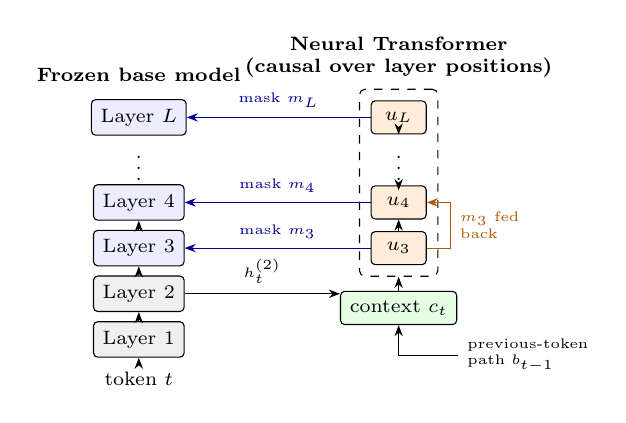
\begin{tikzpicture}[
  font=\scriptsize,
  >={Stealth[length=4pt]},
  lay/.style={draw, rounded corners=1.5pt, minimum width=1.1cm, minimum height=0.42cm, fill=gray!12},
  sp/.style={draw, rounded corners=1.5pt, minimum width=1.1cm, minimum height=0.42cm, fill=blue!7},
  pl/.style={draw, rounded corners=1.5pt, minimum width=0.7cm, minimum height=0.42cm, fill=orange!15},
]
\def\px{3.3}
\node (tok) at (0,-0.5) {token $t$};
\node[lay] (l1) at (0,0) {Layer 1};
\node[lay] (l2) at (0,0.58) {Layer 2};
\node[sp]  (l3) at (0,1.16) {Layer 3};
\node[sp]  (l4) at (0,1.74) {Layer 4};
\node      (ld) at (0,2.28) {$\vdots$};
\node[sp]  (lL) at (0,2.82) {Layer $L$};
\draw[->] (tok) -- (l1);
\draw[->] (l1) -- (l2); \draw[->] (l2) -- (l3); \draw[->] (l3) -- (l4);
\node[font=\scriptsize\bfseries, above=0.1cm of lL] {Frozen base model};
% planner
\node[pl] (p3) at (\px,1.16) {$u_3$};
\node[pl] (p4) at (\px,1.74) {$u_4$};
\node     (pd) at (\px,2.28) {$\vdots$};
\node[pl] (pL) at (\px,2.82) {$u_L$};
\node[draw, dashed, rounded corners=2pt, inner sep=4pt, fit=(p3)(pL)] (planbox) {};
\node[font=\scriptsize\bfseries, above=0.02cm of planbox, align=center] {Neural Transformer\\(causal over layer positions)};
\draw[->] (p3) -- (p4); \draw[->] (p4) -- (pd); \draw[->] (pd) -- (pL);
% seed
\node[draw, rounded corners=1.5pt, fill=green!10] (seed) at (\px,0.4) {context $c_t$};
\draw[->] (l2.east) -- node[above, font=\tiny]{$h^{(2)}_t$} (seed.west |- l2.east);
\node[align=left, font=\tiny, anchor=west] (prev) at (\px+0.75,-0.2) {previous-token\\path $b_{t-1}$};
\draw[->] (prev.west) -| (seed.south);
\draw[->] (seed) -- (planbox.south);
% masks
\draw[->, blue!60!black] (p3.west) -- node[above, font=\tiny]{mask $m_3$} (l3.east);
\draw[->, blue!60!black] (p4.west) -- node[above, font=\tiny]{mask $m_4$} (l4.east);
\draw[->, blue!60!black] (pL.west) -- node[above, font=\tiny]{mask $m_L$} (lL.east);
% feedback
\draw[->, orange!70!black] (p3.east) -- ++(0.3,0) |- node[pos=0.25, right, font=\tiny, align=left]{$m_3$ fed\\back} (p4.east);
\end{tikzpicture}
\caption{The Neural Transformer. After two dense layers, it builds a context vector from the token's hidden state and the previous token's path (its strong neurons), then generates a per-neuron MLP mask for every remaining layer, each conditioned on the masks already chosen. All masks exist before layer~3 runs; attention stays dense.}
\label{fig:overview}
\end{figure}

% ------------------------------------------------------------------------
\section{Related Work}

\paragraph{Predictor-based contextual sparsity.} Deja Vu showed that small, input-dependent subsets of attention heads and MLP neurons reproduce the dense output, and trained per-layer low-rank predictors to select them on OPT models \citep{liu2023dejavu}. ShadowLLM replaced activation-magnitude labels with a gradient-informed importance criterion and a single predictor at the first layer \citep{akhauri2024shadowllm}, again on OPT. Polar Sparsity extends contextual sparsity to batched serving, but applies MLP sparsity only to ReLU models and uses head sparsity alone on SwiGLU models \citep{shrestha2025polar}. These predictors are trained to imitate labels derived from activations; ours is trained on the output of the sparsified model.

\paragraph{Training-free activation sparsity.} CATS, TEAL, R-Sparse and WINA threshold activations or hidden states by magnitude, optionally weighted by weight norms, and reach roughly 40\% to 50\% model-wide sparsity on SwiGLU models with modest loss \citep{lee2024cats,liu2025teal,zhang2025rsparse,chen2026wina}. They decide after the relevant activations are computed, so they cannot schedule weight transfers ahead of a layer. We use magnitude selection with full knowledge of activations as a reference point, not a competitor.

\paragraph{Planning ahead.} GRIFFIN observes that relative activation patterns persist within a sequence and selects one neuron set per sequence from the prompt, which it reuses for every generated token \citep{dong2024griffin}. NeuroPrefetcher predicts, after layer~0, an activation pattern for every downstream layer from a clustered vocabulary of 512 patterns per layer, and uses token-to-token overlap to fetch only new rows from storage \citep{dhar2026neuroprefetcher}. The Neural Transformer also plans ahead, but per token, per neuron, and layer by layer, and it is trained end to end. In mixture-of-experts models, several systems predict future expert choices to prefetch weights, but there the model's own router still decides what runs, so a wrong prediction costs latency rather than quality.

\paragraph{Restoring or building sparsity.} ReLUfication and ProSparse retrain SwiGLU models toward ReLU-like activations \citep{mirzadeh2023relu,song2025prosparse}; MoEfication and LLaMA-MoE convert dense MLPs into experts, the latter with continued pretraining \citep{zhang2022moefication,zhu2024llamamoe}. We leave the base model untouched.

\paragraph{End-to-end gating.} Budget-conditioned gating networks trained with a joint task, consistency and resource objective have been used to skip layers, prune attention heads and shorten reasoning \citep{chen2026e2e}, and Mixture-of-Depths learns per-token layer skipping during pretraining \citep{raposo2024mod}. We apply end-to-end training at neuron granularity in a frozen model and find that adding layer- and group-level gates hurts in this setting (Section~\ref{sec:coarse}).

% ------------------------------------------------------------------------
\section{Method}

\subsection{Problem setup}

Consider a decoder-only transformer with $L$ layers whose MLP blocks use SwiGLU. For a token with MLP input $x$ at layer $l$, the block computes
\begin{equation}
\mathrm{MLP}_l(x) = W^{(l)}_{\mathrm{down}}\Big(\mathrm{SiLU}\big(W^{(l)}_{\mathrm{gate}}x\big) \odot W^{(l)}_{\mathrm{up}}x\Big).
\end{equation}
Neuron $i$ owns row $i$ of the gate and up projections and column $i$ of the down projection. Given a binary mask $m_l$ over the $n$ neurons of layer $l$, the sparse block evaluates only neurons with $m_{l,i}=1$, so in a sparse implementation, skipping a neuron would remove all three of its weight slices from the computation and from memory traffic. In this paper we simulate skipping: the dense block is computed and the masked neurons' contributions are zeroed, which gives the same output as true skipping but no savings (Section~\ref{sec:limits}). We keep attention dense and run the first $d=2$ layers densely. A token's \emph{retention} is the mean of its masks over the $L-d$ sparse layers.

The goal is to choose all masks $m_3,\dots,m_L$ for the current token \emph{before layer 3 executes}, so that the weights a token needs can be scheduled in advance. The base model is frozen throughout.

\subsection{The Neural Transformer}

The Neural Transformer is a small causal transformer whose sequence positions are the base model's sparse layers. It starts from a context vector $c_t$ built from two signals available after layer~2:
\begin{equation}
c_t = W_h\,\frac{h^{(2)}_t}{\mathrm{rms}(h^{(2)}_t)} + \sum_{l=1}^{L} E^{(l)}_{\mathrm{prev}}\, b^{(l)}_{t-1} + v_{\mathrm{prev}}.
\end{equation}
Here $h^{(2)}_t$ is the base model's hidden state for token $t$ after layer~2, normalized by its root-mean-square without a learned scale. The second signal is the \emph{previous-token path}. Each neuron of the previous token is recorded as strong, weak or unobserved: strong if it ran and its absolute activation $|a_i|$ exceeded that neuron's 75th percentile, estimated once from 16 reserved training windows; weak if it ran below that level; unobserved if it was skipped, since its activation was never computed. The bit vector $b^{(l)}_{t-1}$ marks the strong neurons of layer $l$, over all $L$ layers including the two dense ones, so weak and unobserved neurons contribute nothing. Each $E^{(l)}_{\mathrm{prev}}$ is a learned table with one 256-dimensional vector per neuron, so a bit vector is embedded by summing the vectors of its active entries, and $v_{\mathrm{prev}}$ is a learned vector added whenever a previous token exists. No activation magnitudes enter the Neural Transformer.

The Neural Transformer then generates the path one layer at a time. Its input at the position for layer $l$ is the embedding of the mask it chose for layer $l-1$ plus a learned layer-position embedding; a causal transformer with 2 blocks, width 256 and 4 attention heads produces a state $u_l$, and a per-layer head maps it to one score per neuron:
\begin{equation}
s_l = W^{(l)}_{\mathrm{out}}\,u_l, \qquad m_l = \mathbb{1}\big[s_l \ge \tau_l\big].
\end{equation}
Each layer's mask is thus conditioned on the context and on every mask chosen before it, and no information from the current token's later layers is used. In practice the cutoff for layer $l$ is $\tau_l=o_l+\delta$: per-layer offsets $o_l$ are set at the start of end-to-end training so that each layer initially keeps the target fraction, and a single shift $\delta$ is calibrated on validation documents so that mean retention matches the target. Throughout, \emph{target} is the fraction a threshold is calibrated toward and \emph{retention} is the fraction actually kept, which we always report as measured. Individual tokens and layers still keep different numbers of neurons. The parameters are dominated by per-neuron tables: $L$ previous-path tables, $L-d-1$ mask tables and $L-d$ output heads, each of size $n\times w$ for width $w$. The shared transformer has only 1.58M parameters (feed-forward width 1,024). In total the Neural Transformer has 126.5M parameters for Qwen3-1.7B and 337.0M for Mistral-7B.

\subsection{Training objective}

We train the Neural Transformer through the frozen base model by comparing a dense teacher pass with a gated student pass on the same text. With final hidden states $h_T$ and $h_S$ (before the final normalization), next-token distributions $p_T$ and $p_S$, and gates $g$, the loss is
\begin{equation}
\mathcal{L} = -\ln\max\big(\cos(h_T, h_S),\varepsilon\big) + \beta\,\mathrm{KL}\big(p_T \,\|\, p_S\big) + \frac{\alpha}{|\mathcal{N}|}\sum_{i \in \mathcal{N}} g_i,
\end{equation}
where $\mathcal{N}$ is the set of gateable neurons across the sparse layers, averaged over all token positions. We use $\varepsilon=0.01$ and $\beta=1$. The first two terms preserve the output; the third prices compute. Rather than fixing $\alpha$, we adjust it by dual ascent toward a target mean retention $r^\ast$: after each step, $\alpha\leftarrow\min\big(100,\max(0,\alpha+0.05(\bar r-r^\ast))\big)$, where $\bar r$ is the batch's retention.

Gates are binary in every forward pass, so the base model always sees masks of the kind it sees at inference; gradients flow through the relaxed sigmoid $\sigma(s/T)$ by a straight-through estimator \citep{bengio2013ste}, with $T$ annealed from 1.0 to 0.1. Early in training, logistic (binary-Concrete) noise is added to the scores before thresholding \citep{jang2017gumbel}, so borderline neurons are explored; later the gates are deterministic. On Qwen3-1.7B the last 20\% of each run is deterministic. On Mistral-7B, the 50\% phase becomes deterministic after 20M of its 25M tokens, the 40\% phase after 8M of 15M, and the 30\% and 20\% phases are deterministic throughout. A Qwen ablation training with deterministic gates from the first step gave +8.19\% versus +8.60\% at matched retention, with a paired 95\% interval of $[-1.06, +0.23]$ points, so the noise schedule is not critical.

\subsection{Training procedure}

Training proceeds in three stages.
\begin{itemize}
\item \textbf{Imitation warm start (10M tokens).} With teacher forcing, the Neural Transformer predicts, for each layer, the oracle mask that keeps the neurons with the largest absolute activations at the target, under binary cross-entropy with positive examples weighted 2. Targets alternate between 50\% and 40\%. During this stage the previous-token path is privileged: the dense model's strong neurons, restricted to the oracle mask.
\item \textbf{Scheduled sampling (2M tokens on Mistral, 1M on Qwen).} The oracle masks fed back as inputs are gradually replaced by the Neural Transformer's own choices \citep{bengio2015scheduled}, so that it learns to recover from its own errors.
\item \textbf{End-to-end training.} The Neural Transformer generates every path from its own choices and is trained with the objective above.
\end{itemize}
Because tokens are processed in parallel during training, the previous-token path is not available within a single pass. Each batch therefore runs a gradient-free gated pass, without previous-token paths, to record every token's path, followed by the training pass that uses the previous token's recorded path. This two-pass scheme approximates inference rather than reproducing it: at inference, each token's recorded path comes from a pass that itself used its predecessor's path, a chain the single recording pass cannot reproduce exactly.

To reach low retention, we train one Neural Transformer on a curriculum of targets, each phase continuing from the previous checkpoint: on Mistral-7B, 25M tokens with a 50\% target, 15M at 40\%, and 10M each at 30\% and 20\%: 60M end-to-end token presentations in total, after 12M token presentations of imitation warm start. For the 40\%, 30\% and 20\% phases, training was extended (from 10M to 15M tokens at 40\%, and from 5M to 10M at 30\% and 20\%) only if validation KL had improved by at least 0.001; each extension met this rule. We call the resulting Mistral checkpoints NT-50, NT-40, NT-30 and NT-20 after their training targets. After each phase, the shift $\delta$ is calibrated on 24 held-out validation documents. On Qwen3-1.7B the Neural Transformer instead receives 2M end-to-end tokens per target, in independent branches from the same warm start.

% ------------------------------------------------------------------------
\section{Experimental Setup}

\paragraph{Models.} Our main model is Mistral-7B-v0.1 \citep{jiang2023mistral}: 32 layers, 14,336 MLP neurons per layer, hidden size 4,096. Development and analysis use Qwen3-1.7B-Base \citep{yang2025qwen3}: 28 layers, 6,144 MLP neurons per layer, hidden size 2,048. Both use SwiGLU MLPs and grouped-query attention, and both stay frozen.

\paragraph{Data.} Neural Transformers are trained on 512-token windows from FineWeb-Edu (web), codeparrot-clean (code) and UltraChat-200k (conversation) in an 80/10/10 token ratio, with document-level splits. Thresholds are calibrated on 24 separate validation documents (8 per domain). Test results use a fixed set of 63 held-out documents (24 web, 15 code, 24 conversation), one window of 128--512 Qwen tokens each, scoring 28,857 positions on Qwen3-1.7B and 34,000 positions on Mistral-7B after retokenization. The same set is reused across experiments, so it is exploratory rather than a single-use test set.

\paragraph{Sparsity and retention.} Unless stated otherwise, the first two layers and all attention blocks are dense, and a mask covers an inactive neuron's gate, up and down weights. All results simulate skipping by masking a dense computation, so they measure quality at a given retention, not speed. Retention is the measured fraction of eligible neurons kept in the sparse layers, reported as realized on the test set rather than as the target.

\paragraph{Evaluation protocols.}
\begin{itemize}
\item \emph{Whole-document perplexity:} every token is scored with the sparse model.
\item \emph{Prompt continuation:} a prompt is processed densely, and only the continuation is sparse and scored (the first continuation token is predicted from the dense prompt and is excluded). This is the setting GRIFFIN is designed for. We use 64-token prompts on the 63 test documents, and 512- or 1,024-token prompts on 64 WikiText-2 test windows of 1,536 tokens whose final 512 tokens are scored; both prompt lengths score identical targets, and thresholds for this setting are calibrated on the WikiText-2 validation split.
\item \emph{NeuroPrefetcher's configuration:} 20 dense layers and a dense down projection, as in its published quality results.
\item \emph{HellaSwag} \citep{zellers2019hellaswag}: all 10,042 validation examples, zero-shot, with length-normalized accuracy. Retention is calibrated on 1,024 unlabeled training examples. The context is processed densely and its final logits score the first answer token; for an ending of $L$ tokens, the remaining $L-1$ likelihood terms come from sparse forward passes over the answer tokens. GRIFFIN's paper instead sparsifies only the final token's forward pass, a milder setting.
\end{itemize}
We report the change in perplexity relative to the dense model, KL divergence, next-token agreement with the dense model, and paired document-bootstrap 95\% confidence intervals.

\paragraph{Baselines.} \emph{GRIFFIN} selects, per sequence, the neurons with the largest relative activations in the dense prompt and reuses them for every subsequent token \citep{dong2024griffin}. We reimplement its official selection statistic (the norm across prompt positions of per-token normalized activations) in our harness, with the same dense first two layers as the Neural Transformer. \emph{NeuroPrefetcher} \citep{dhar2026neuroprefetcher} is evaluated with the authors' released Mistral-7B predictor and pattern vocabulary; we reproduce the reference WikiText perplexities saved in their code release (dense 3.9934 versus 3.9937; 20 dense layers at their 50\% setting, 5.6888 versus 5.6903). On Qwen3-1.7B we reimplement it. As references that decide after seeing activations, we report greedy magnitude selection and TEAL- and WINA-style selection restricted to MLP neurons. Baselines are calibrated to the same retention as the Neural Transformer wherever possible; residual differences are reported.

\paragraph{Compute.} Qwen3-1.7B experiments ran on single NVIDIA A40 GPUs at \$0.59 per hour; recorded estimates for individual runs range from about \$0.13 to \$8, and a reconciled total is not yet available. The Mistral-7B Neural Transformer was trained on single NVIDIA A100 80GB GPUs in three allocations. Imitation, scheduled sampling and the first 10M tokens at 50\% took about 7.1 GPU-hours of training at \$1.79 per hour (no posted charge recorded); the rest of the 50\% phase and the 40\% phase cost \$49.09 in posted charges; and the 30\% and 20\% phases took about 24 GPU-hours of training at \$2.09 per hour, roughly \$50 (posted charges not yet reconciled). Evaluations used A100 and H200 GPUs.

% ------------------------------------------------------------------------
\section{Results}

\subsection{Perplexity against planning-ahead baselines}

The Neural Transformer keeps perplexity within 5.2\% of the dense model at about half of the MLP neurons, while GRIFFIN and NeuroPrefetcher increase it by 72\% and 228\% (Table~\ref{tab:ppl}). The gap holds when GRIFFIN is given its preferred setting of long dense prompts: on WikiText-2 with 1,024 prompt tokens, the Neural Transformer's increase is 10.5\% against 66.6\% for GRIFFIN and 157.4\% for NeuroPrefetcher at about 48\% retention. Without any prompt, scoring whole documents with two dense layers, the released NeuroPrefetcher predictor raises perplexity by 277.6\% at 48.06\% retention, against 5.41\% at 49.49\% for the Neural Transformer.

\begin{table}[t]
\centering
\caption{Mistral-7B, prompt-continuation protocol: perplexity increase over the dense model on the continuation (lower is better). 64-token rows use the 63 test documents, where the Neural Transformer's retention was 1.1--1.2 percentage points higher than the baselines' (49.15\% and 41.27\%). 512- and 1,024-token rows use WikiText-2 windows with identical scored tokens, at 48\% and 40\% targets for the baselines and 48.2--48.4\% and 40.3\% retention for the Neural Transformer. Compare the 64-token rows with the others only within a row.}
\label{tab:ppl}
\small
\setlength{\tabcolsep}{4pt}
\begin{tabular}{@{}llrrr@{}}
\toprule
Prompt & Target & NT & GRIFFIN & NeuroPref. \\
\midrule
\multirow{2}{*}{64}    & 50\%    & \textbf{+5.21} & +72.47  & +227.96 \\
                        & 40\%    & \textbf{+7.29} & +117.10 & +594.59 \\
\addlinespace
\multirow{2}{*}{512}   & $\sim$48\% & \textbf{+10.62} & +71.44  & +169.76 \\
                        & $\sim$40\% & \textbf{+14.52} & +114.00 & +490.90 \\
\addlinespace
\multirow{2}{*}{1,024} & $\sim$48\% & \textbf{+10.50} & +66.62  & +157.45 \\
                        & $\sim$40\% & \textbf{+14.10} & +106.48 & +475.13 \\
\bottomrule
\end{tabular}
\end{table}

Because the 512- and 1,024-token runs score the same WikiText-2 tokens, doubling the dense prompt is a controlled comparison: it lowers GRIFFIN's increase from 71.4\% to 66.6\% and the Neural Transformer's only from 10.6\% to 10.5\%. A follow-up on the same WikiText-2 tokens with fixed offsets rules out long context as the cause of the Neural Transformer's larger increase there: moving from a 64-token to a 1,024-token prompt changes it only from +10.29\% to +10.89\% at 50\%, an excess of 0.005 nats per token (95\% interval $[0.001, 0.010]$), and not significantly at 40\%. The difference from the 64-token document setting therefore reflects the dataset. Within each continuation, retention drifts downward (NT-50 with a 64-token prompt, from about 57\% over the first 32 continuation tokens to about 48\% over the last 32) while per-token excess loss rises.

In NeuroPrefetcher's own configuration (20 dense layers, dense down projection, 50\% target), the Neural Transformer increases perplexity by 5.75\% at 48.70\% retention, against 38.61\% at 49.66\% for NeuroPrefetcher. On the authors' own 2,048-token WikiText slice, the released predictor gives +42.5\% at 49.63\% retention, reproducing the 5.69 versus 3.99 reference perplexities saved in the authors' release. In a comparably relaxed configuration on Qwen3-1.7B (dense down projection and a larger dense prefix), the Neural Transformer gives +1.30\% at 50.76\% retention against +181\% at 50.00\% for our reimplementation.

\subsection{Downstream accuracy at matched retention}

On HellaSwag, the Neural Transformer stays within 2.1 points of the dense model down to 40\% retention, while GRIFFIN and NeuroPrefetcher lose 10.3 and 28.6 points (Table~\ref{tab:hellaswag}). At 29.70\% retention, NT-30 (77.09\%) still scores higher than GRIFFIN at 48.05\% (74.10\%), and at 19.74\% retention NT-20 scores 73.99\%, statistically indistinguishable from GRIFFIN at 48.05\% (paired difference $-0.11$ points, 95\% interval $[-0.77, +0.53]$) while keeping 2.4 times fewer neurons.

\begin{table}[t]
\centering
\caption{Mistral-7B, HellaSwag normalized accuracy (\%) on 10,042 examples; dense model 81.18. Change from dense in parentheses; retention in the second line of each row.}
\label{tab:hellaswag}
\small
\setlength{\tabcolsep}{3.5pt}
\begin{tabular}{@{}lccc@{}}
\toprule
Target & NT & GRIFFIN & NeuroPref. \\
\midrule
\multirow{2}{*}{$\sim$48\%} & \textbf{79.49} (\textminus1.69) & 74.10 (\textminus7.08) & 60.92 (\textminus20.25) \\
 & {\footnotesize 47.65\%} & {\footnotesize 48.05\%} & {\footnotesize 47.97\%} \\
\addlinespace
\multirow{2}{*}{$\sim$40\%} & \textbf{79.11} (\textminus2.07) & 70.93 (\textminus10.25) & 52.55 (\textminus28.63) \\
 & {\footnotesize 39.66\%} & {\footnotesize 40.04\%} & {\footnotesize 40.04\%} \\
\addlinespace
\multirow{2}{*}{$\sim$30\%} & \textbf{77.09} (\textminus4.09) & -- & -- \\
 & {\footnotesize 29.70\%} & & \\
\addlinespace
\multirow{2}{*}{$\sim$20\%} & \textbf{73.99} (\textminus7.19) & -- & -- \\
 & {\footnotesize 19.74\%} & & \\
\bottomrule
\end{tabular}
\end{table}

GRIFFIN's own paper reports near-zero HellaSwag loss under its final-token-only protocol. In ours, $L-1$ of the $L$ likelihood terms of each ending come from sparse forward passes (Section~4), so our GRIFFIN numbers are not comparable with its published ones.

\subsection{Quality across targets}

A single Neural Transformer trained on the target curriculum degrades smoothly from 51\% to 21\% retention, with no collapse (Figure~\ref{fig:budget}). At 31.48\% retention, where the masks exclude roughly half of Mistral-7B's total weights, perplexity rises 12.50\% and the sparse model's top next-token prediction agrees with the dense model's 85.56\% of the time. At 41.49\% retention, perplexity rises 7.80\% (95\% interval 7.25\% to 8.32\%). At 21.46\% retention, it rises 21.31\% (95\% interval 20.16\% to 22.47\%) with 81.97\% agreement.

\begin{figure}[t]
\centering
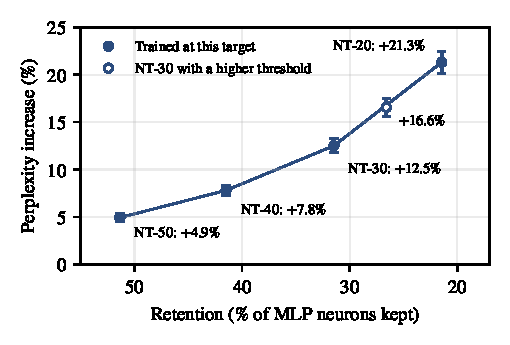
\includegraphics[width=\columnwidth]{budget_curve.pdf}
\caption{Perplexity increase of the Mistral-7B Neural Transformer as retention falls (whole-document protocol, test set), from one model trained on a 50\%\,$\to$\,40\%\,$\to$\,30\%\,$\to$\,20\% curriculum. The hollow point reuses NT-30 with a higher threshold; bars are 95\% bootstrap intervals.}
\label{fig:budget}
\end{figure}

The 26.61\% point reuses NT-30 with a higher threshold and was never trained at that target. Validation curves suggest that further training could still help at the lowest targets: between 5M and 10M tokens, validation perplexity increase fell from 12.8\% to 12.1\% at 30\% and from 23.2\% to 21.5\% at 20\%. At 40\% the curve had flattened (+7.48\% at 10M, +7.28\% at 15M). At 50\%, the drop from +8.04\% at 20M tokens to +4.85\% at 25M coincides with the switch to deterministic gates at 20M, so it cannot be attributed to training length alone.

\subsection{Results on Qwen3-1.7B}

On Qwen3-1.7B, the Neural Transformer increases whole-document perplexity by 8.6\% at 51.62\% retention and 15.7\% at 41.14\%, where our NeuroPrefetcher reimplementation reaches 62.16 and 368.88 perplexity against 5.89 dense. Under the continuation protocol of Section~\ref{sec:prior}, which scores different tokens and is not comparable with these whole-document numbers, additional training and a sequence prior lower its increase at the 50\% target from +7.71\% to +6.48\% and +6.02\%. The smaller model is harder to sparsify throughout: the same method costs less on Mistral-7B at every target we measured.

% ------------------------------------------------------------------------
\section{Analysis and Ablations}

All analyses in this section use Qwen3-1.7B, MLP-only sparsity and the whole-document protocol unless noted.

\subsection{End-to-end training versus imitation}

Training on output fidelity, rather than on activation labels, accounts for most of the Neural Transformer's quality. Table~\ref{tab:e2e} isolates this with simpler \emph{layer-ahead predictors}, which choose the mask for layer $l+2$ from information available at layer $l$. One reads the hidden state; the other reads the previous-token path. Each is trained either by imitating magnitude-oracle masks or end to end with the objective of Section~3.3.

\begin{table}[t]
\centering
\caption{Qwen3-1.7B, layer-ahead predictors: perplexity increase (\%) at matched mean retention. Rows in italics decide after observing activations and cannot run ahead of time.}
\label{tab:e2e}
\small
\setlength{\tabcolsep}{4pt}
\begin{tabular}{@{}lrr@{}}
\toprule
Selector & 50\% target & 40\% target \\
\midrule
Fixed selection (same for all tokens) & +2,259 & +3,653 \\
\addlinespace
Previous-token-path input, imitation & +23.16 & +38.32 \\
Hidden-state input, imitation & +18.85 & +30.48 \\
\addlinespace
Previous-token-path input, end to end & +3.86 & +6.49 \\
Hidden-state input, end to end & \textbf{+2.64} & \textbf{+4.75} \\
\midrule
\textit{Greedy magnitude (activations known)} & \textit{+0.96} & \textit{+2.39} \\
\textit{TEAL-style, MLP only} & \textit{+0.99} & \textit{+2.05} \\
\textit{WINA-style, MLP only} & \textit{+1.03} & \textit{+2.64} \\
\bottomrule
\end{tabular}
\end{table}

End-to-end training reduces the cost of both predictors by a factor of 6 to 7 at 50\% retention. Imitation fails because its loss weights every neuron equally, whereas the output depends mostly on the largest contributions, and because errors compound across layers in ways that per-layer labels never expose. The references decide after observing activations and are not achievable in advance; they bound what greedy selection can reach, not what a learned selector can reach.

\subsection{Layer-by-layer generation versus one-shot prediction}
\label{sec:oneshot}

The Neural Transformer's central design choice is to generate the path one layer at a time, each mask conditioned on the masks already chosen. To test it, we compare it with one-shot controls that use the same transformer but receive the context vector $c_t$ at every layer position and predict all masks at once, with no mask feedback. They follow the same recipe (10M imitation, 1M scheduled-sampling and 2M end-to-end tokens per target) and are calibrated the same way (Table~\ref{tab:oneshot}).

\begin{table}[t]
\centering
\caption{Qwen3-1.7B, whole-document protocol: perplexity increase (\%) of upfront predictors after layer~2, with test retention in parentheses. ``Prev.-token path'' is the previous-token path of Section~3.2.}
\label{tab:oneshot}
\small
\begin{tabular}{@{}lrr@{}}
\toprule
Upfront predictor & 50\% target & 40\% target \\
\midrule
One-shot, hidden state only & +90.47 {\footnotesize (49.9)} & +113.55 {\footnotesize (40.0)} \\
One-shot, hidden + prev.-token path & +12.37 {\footnotesize (51.1)} & +22.20 {\footnotesize (40.9)} \\
Layer by layer (NT) & \textbf{+8.60} {\footnotesize (51.6)} & \textbf{+15.70} {\footnotesize (41.1)} \\
NT, prev.-token path removed & +25.64 {\footnotesize (50.8)} & +38.36 {\footnotesize (40.8)} \\
\addlinespace
\multicolumn{3}{@{}l}{\emph{Second training seed}} \\
One-shot, hidden + prev.-token path & +12.07 {\footnotesize (51.1)} & +21.43 {\footnotesize (41.4)} \\
Layer by layer (NT) & \textbf{+8.67} {\footnotesize (51.4)} & \textbf{+15.40} {\footnotesize (41.1)} \\
\bottomrule
\end{tabular}
\end{table}

With identical inputs, generating the path layer by layer lowers the perplexity increase by 3.8 points at 50\% and 6.5 points at 40\% relative to one-shot prediction, so conditioning each layer on earlier choices matters more as retention falls. The previous-token path is the larger factor: a one-shot predictor without it collapses (+90\%), and removing it from the trained Neural Transformer at evaluation, with thresholds recalibrated to the same retention, triples its cost at 50\% (+25.6\% versus +8.6\%). A second training seed, with a new initialization and the same data order, replicates both conclusions: the Neural Transformer beats the one-shot model by 3.4 and 6.0 points (paired intervals $[2.4, 4.4]$ and $[4.6, 7.6]$), and end-to-end training again beats imitation for both layer-ahead predictors. The previous-token-path ablations use the first seed only.

\subsection{Granularity: neurons versus groups and patterns}

Per-token sparsity in SwiGLU models lives at the level of individual neurons. With magnitude selection and activations known, keeping 50\% of single neurons costs 1.12\% in perplexity (KL 0.0136 nats per token, 94.76\% next-token agreement). Keeping 50\% of neuron groups, selected by their exact contribution to the output, costs 22.5\%, 28.3\% and 37.1\% for groups of 16, 32 and 128 neurons. The two comparisons use different selection scores, so this is not a perfectly isolated test of granularity, but the gap is more than an order of magnitude. Re-clustering neurons from scratch by co-activation, with about 98\% of new groups crossing the old boundaries, improved perplexity by at most 1.02\% relative, leaving 50\%-retention groups 22\% to 27\% above dense. Each token's important neurons cut across any fixed grouping.

Clustered activation vocabularies fail for the same reason. Replacing NeuroPrefetcher's predictor with the true nearest of its 512 patterns per layer changes perplexity at 50\% retention only from 78.03 to 76.57 (dense 5.89). The pattern vocabulary, not the predictor, limits it once skipping covers most of the model.

\subsection{Planning ahead versus layer-ahead prediction}

Committing to a token's whole path after layer~2 costs quality relative to layer-ahead prediction, which observes the token's hidden state at every layer: on Qwen3-1.7B at the 50\% target, the layer-ahead predictor with hidden-state input reaches +2.64\%, against +8.6\% at 51.62\% retention for the Neural Transformer under the same protocol, although the two predictors also differ in training length (13M versus 2M end-to-end tokens). Part of the gap is the price of lead time, which layer-ahead prediction cannot offer beyond a layer or two.

We also compared what each input carries. In early imitation probes on 128-neuron groups at a 25\% target, a previous-token path with one bit per group recovered about 80\% of the predictive signal of the hidden state (normalized scores of 0.514 versus 0.641, where 0 is chance and 1 is perfect), and exact magnitudes added nothing over the bits (0.517). After end-to-end training at the neuron level, the hidden-state input remained ahead by 1.22 and 1.74 points at 50\% and 40\% retention (95\% intervals $[0.82, 1.58]$ and $[1.22, 2.27]$).

\subsection{Sequence-level prior}
\label{sec:prior}

We adapt GRIFFIN's sequence statistic to sparse execution. For each neuron that ran, we accumulate its squared activation divided by the sum of squared activations of the observed neurons in that layer, weighting dense-prompt tokens by 4; the per-layer log-RMS of these values is standardized, clipped to $\pm 8$, and reset at each document. Skipped neurons are left neutral. The score enters the Neural Transformer's output as a learned per-layer gain and bias (52 parameters). Starting from the trained Neural Transformer, this gives a small further gain over a control trained for the same 2M additional tokens (Table~\ref{tab:prior}). Initializing from the prior instead, by zeroing the output heads, performs poorly.

\begin{table}[t]
\centering
\caption{Qwen3-1.7B Neural Transformer, perplexity increase (\%) after calibration, continuation protocol: each 512-token window starts with a dense 64-token prompt that is not scored. Not comparable with the whole-document numbers elsewhere in this section. ``NT'' is the trained model remeasured without further training.}
\label{tab:prior}
\small
\begin{tabular}{@{}lrr@{}}
\toprule
Variant & 50\% target & 40\% target \\
\midrule
NT & +7.71 & +13.77 \\
NT, equal additional training & +6.48 & +12.33 \\
NT + sequence prior & \textbf{+6.02} & \textbf{+11.12} \\
Prior-first initialization & +44.23 & +70.09 \\
\bottomrule
\end{tabular}
\end{table}

At 50\%, the prior beats the equal-training control by 0.46 points while keeping slightly fewer neurons (51.24\% versus 51.53\%); the paired interval favors the prior, but this is a single seed. At 40\%, the prior beats the control by 1.21 points (+11.12\% versus +12.33\%, the control keeping 40.95\%). The Mistral-7B results in Section~5 do not use the prior.

\subsection{Coarser gates and attention}
\label{sec:coarse}

Offering coarse options in addition to neurons did not help. At roughly matched total compute, a layer-ahead predictor with hidden-state input and neuron gates alone reached +3.02\%; adding layer gates gave +6.48\%, adding 128-neuron group gates gave +9.10\%, and with all three levels the trained checkpoint reached +10.49\% at its training-time threshold but +1,145.15\% after the threshold was recalibrated to the target retention. This points to calibration instability, where a small threshold change switches off whole layers or groups, rather than to failed training. The compute penalty pushes hardest on the coarsest gates, since one such decision saves the most compute.

Attention is more fragile than the MLP. With activations known, keeping 75\% of attention heads cost 14.1\% in perplexity and keeping 50\% cost 344\%, reduced to 9.7\% and 79\% when the first and last two layers were kept dense. We therefore keep attention dense throughout.

% ------------------------------------------------------------------------
\section{Deployment Checks}
\label{sec:deploy}

We ran three preregistered checks of whether the quality results carry over to harder tasks and to real execution, on Mistral-7B with NT-30 and NT-20, batch size one, cached decoding, and attention and the first two layers dense. Each used one A100 80GB GPU.

\paragraph{Reasoning benchmarks.} On GSM8K (all 1,319 test problems, 8-shot, greedy, strict final-answer match) and MMLU (all 14,042 test questions, 5-shot), the prompt is dense except its final token, and every generated token is sparse. Accuracy falls substantially (Table~\ref{tab:reason}). Retention, however, is about half the target: thresholds calibrated on our validation documents keep only 15\% and 10\% of neurons on GSM8K generations and 13\% and 8\% on MMLU's answer token. These results therefore measure both sparsity and a failure of calibration to transfer across input formats. On GSM8K's reference solutions, teacher-forced perplexity rises 11.2\% at 20.8\% retention, far less than the drop in generated accuracy, consistent with errors that compound through multi-step generation.

\begin{table}[t]
\centering
\caption{Mistral-7B reasoning accuracy (\%), single seed. Retention in parentheses; gap to dense with paired-bootstrap 95\% interval.}
\label{tab:reason}
\small
\setlength{\tabcolsep}{3pt}
\begin{tabular}{@{}lccc@{}}
\toprule
 & Dense & NT-30 & NT-20 \\
\midrule
GSM8K & 40.49 & 15.16 {\footnotesize (15.2)} & 8.87 {\footnotesize (10.2)} \\
 gap & & $-25.3$ {\footnotesize $[-28.1,-22.4]$} & $-31.6$ {\footnotesize $[-34.4,-29.0]$} \\
\addlinespace
MMLU & 62.42 & 55.99 {\footnotesize (13.2)} & 53.13 {\footnotesize (8.4)} \\
 gap & & $-6.4$ {\footnotesize $[-7.2,-5.7]$} & $-9.3$ {\footnotesize $[-10.1,-8.5]$} \\
\bottomrule
\end{tabular}
\end{table}

\paragraph{Latency and weight traffic.} We timed decoding of 64 WikiText-2 tokens over eight blocks, including the Neural Transformer, row and column gathering, transfers and scheduling (Table~\ref{tab:latency}). With all weights on the GPU, a straightforward PyTorch implementation decodes at 0.44--0.47 times dense speed. When MLP weights are streamed from CPU memory, the plan cuts the weight payload per token from 11.3\,GB to 5.4\,GB and 4.0\,GB (52\% and 65\% less), yet decoding is still slower than streaming the dense model, because the Neural Transformer's 30 sequential steps and per-row gathers cost more than the bytes saved. Gathered and masked execution also differ slightly numerically in BF16 (maximum logit difference 4.9; top-1 agreement 93--96\% per arm). These are feasibility measurements of an unoptimized implementation, not a bound on what fused kernels and overlapped planning could achieve.

\begin{table}[t]
\centering
\caption{Mistral-7B decode speed relative to dense in the same memory setting (paired-bootstrap 95\% interval), with retention and measured CPU-to-GPU weight payload per token. Dense: 27.2 tokens/s on GPU, 1.03 tokens/s with CPU-resident MLP weights.}
\label{tab:latency}
\small
\setlength{\tabcolsep}{3pt}
\begin{tabular}{@{}llccc@{}}
\toprule
Weights & Arm & Retention & Speed & Payload \\
\midrule
GPU & NT-30, masked & 44.2\% & 0.47$\times$ & -- \\
GPU & NT-30, gathered & 44.1\% & 0.44$\times$ & -- \\
GPU & NT-20, gathered & 30.8\% & 0.44$\times$ & -- \\
\addlinespace
CPU & dense & 100\% & 1.00$\times$ & 11.3\,GB \\
CPU & NT-30, gathered & 44.1\% & 0.40$\times$ {\footnotesize [0.36, 0.44]} & 5.4\,GB \\
CPU & NT-20, gathered & 30.7\% & 0.61$\times$ {\footnotesize [0.52, 0.73]} & 4.0\,GB \\
\bottomrule
\end{tabular}
\end{table}

\paragraph{Self-speculative decoding.} Using the masked model (NT-30 or NT-20) as its own draft for dense greedy verification, with drafts of 4 or 8 tokens on 16 WikiText-2 blocks, 2.6 to 4.4 drafted tokens are accepted per verification (51--71\% of proposals). Because the draft is computed as a masked dense model, decoding is 0.25--0.32 times dense speed, and the emitted tokens did not exactly match dense greedy decoding in every block, for reasons not yet resolved. We therefore make no speedup or lossless-output claim; the acceptance rates suggest the idea is worth revisiting with a genuinely sparse draft.

% ------------------------------------------------------------------------
\section{Limitations}\label{sec:limits}

\paragraph{No speedup yet.} Except for the deployment checks, all experiments compute the dense model and apply masks, so they establish quality at a given retention. The one timed implementation is slower than dense decoding (Section~\ref{sec:deploy}). The Neural Transformer's own cost is not negligible: 126.5M parameters on Qwen3-1.7B and 337.0M on Mistral-7B. Counting every table product as a dense matrix multiplication, it costs about 10\% of Qwen3-1.7B's per-token compute and about 5\% of Mistral-7B's; implementing the table products as gathers of the active columns reduces this, but its 30 sequential steps per token add latency that must be overlapped with the base model's layers. Fused gather kernels, a faster Neural Transformer, overlap with the base model and asynchronous prefetching are needed before any net gain can be claimed.

\paragraph{Retention does not transfer across formats.} A threshold calibrated on general text realizes very different retention on other inputs: about half the target on GSM8K and MMLU, and more than the target on WikiText-2 decoding. A per-token budget or task-specific calibration is needed before low-retention checkpoints can be deployed, and the large GSM8K drop shows that multi-step reasoning is much more sensitive than perplexity suggests. We evaluate two models.

\paragraph{Seeds.} The central Qwen ablations (layer by layer versus one-shot, and end-to-end versus imitation) are replicated in two training seeds, which is too few to estimate seed variance. All Mistral-7B results come from one training run. Document-level confidence intervals capture evaluation noise, not seed variation.

\paragraph{Batch size one.} Contextual sparsity loses its benefit at large batch sizes, because the union of neurons needed by different sequences approaches the full layer \citep{shrestha2025polar}. Our setting is single-sequence inference, such as on-device or memory-constrained deployment.

\paragraph{Baseline fidelity.} On Mistral-7B, NeuroPrefetcher uses the authors' released artifacts, whose saved reference perplexities we reproduce. On Qwen3-1.7B it is our reimplementation, whose pattern-prediction accuracy (61.42\% for gate and 48.81\% for up patterns) is far below the roughly 99\% reported for Mistral; the nearest-pattern ablation shows this accuracy gap does not explain its collapse.

% ------------------------------------------------------------------------
\section{Conclusion}

A token's full MLP neuron path in a frozen SwiGLU model can be planned after two dense layers with small quality loss. The Neural Transformer generates per-neuron masks layer by layer and is trained end to end on output fidelity; on Mistral-7B it keeps perplexity within 5.2\% of the dense model at about half of the neurons and loses 2.1 HellaSwag points at 40\%, where GRIFFIN and NeuroPrefetcher degrade by an order of magnitude more. Two findings explain the gap: training on the sparsified model's output, rather than on activation labels, cuts the cost of a predictor by 6 to 7 times, and per-token sparsity in these models lives at the level of single neurons, which fixed groups and pattern vocabularies discard. Our deployment checks show what remains: calibration that holds across input formats, and an implementation whose reduced weight traffic actually becomes faster decoding. Both are necessary before the quality shown here can turn into savings in memory-constrained inference.

\paragraph{Acknowledgments and AI disclosure.} The author used Claude (Anthropic) to help draft and edit the text and to write experiment code. The author designed the study, ran the experiments and checked every reported number against the raw results, and takes full responsibility for the content.

% ------------------------------------------------------------------------
\small
\setlength{\bibsep}{2pt plus 1pt}
\begin{thebibliography}{30}

\bibitem[Akhauri et~al.(2024)]{akhauri2024shadowllm}
Akhauri, Y., AbouElhamayed, A.~F., Dotzel, J., Zhang, Z., Rush, A.~M., Huda, S., and Abdelfattah, M.~S.
\newblock ShadowLLM: Predictor-based contextual sparsity for large language models.
\newblock In \emph{Proceedings of EMNLP}, 2024.

\bibitem[Alizadeh et~al.(2024)]{alizadeh2024flash}
Alizadeh, K., Mirzadeh, I., Belenko, D., Khatamifard, K., Cho, M., Del~Mundo, C.~C., Rastegari, M., and Farajtabar, M.
\newblock LLM in a flash: Efficient large language model inference with limited memory.
\newblock In \emph{Proceedings of ACL}, 2024.

\bibitem[Bengio et~al.(2015)]{bengio2015scheduled}
Bengio, S., Vinyals, O., Jaitly, N., and Shazeer, N.
\newblock Scheduled sampling for sequence prediction with recurrent neural networks.
\newblock In \emph{Advances in Neural Information Processing Systems}, 2015.

\bibitem[Bengio et~al.(2013)]{bengio2013ste}
Bengio, Y., L{\'e}onard, N., and Courville, A.
\newblock Estimating or propagating gradients through stochastic neurons for conditional computation.
\newblock arXiv:1308.3432, 2013.

\bibitem[Chen et~al.(2026a)]{chen2026wina}
Chen, S., Zhao, D., Ko, J., Banbury, C., Zhuang, H., Liang, L., Cameron, P., and Chen, T.
\newblock WINA: Weight informed neuron activation for accelerating large language model inference.
\newblock In \emph{ICLR}, 2026.

\bibitem[Chen et~al.(2026b)]{chen2026e2e}
Chen, Y., Duan, J., Zhang, R., et~al.
\newblock End-to-end dynamic sparsity for resource-adaptive LLM inference.
\newblock arXiv:2606.27743, 2026.

\bibitem[Dhar et~al.(2026)]{dhar2026neuroprefetcher}
Dhar, N., Islam, M.~R., Zhang, X., Sun, G., Islam, S., Deng, B., and Suo, K.
\newblock NeuroPrefetcher: Storage-aware sparse LLM inference via delta prefetching.
\newblock In \emph{Proceedings of the 55th International Conference on Parallel Processing (ICPP)}, 2026. arXiv:2608.22643.

\bibitem[Dong et~al.(2024)]{dong2024griffin}
Dong, H., Chen, B., and Chi, Y.
\newblock Prompt-prompted adaptive structured pruning for efficient LLM generation.
\newblock In \emph{Conference on Language Modeling (COLM)}, 2024.

\bibitem[Jang et~al.(2017)]{jang2017gumbel}
Jang, E., Gu, S., and Poole, B.
\newblock Categorical reparameterization with Gumbel-softmax.
\newblock In \emph{ICLR}, 2017.

\bibitem[Jiang et~al.(2023)]{jiang2023mistral}
Jiang, A.~Q., Sablayrolles, A., Mensch, A., et~al.
\newblock Mistral 7B.
\newblock arXiv:2310.06825, 2023.

\bibitem[Lee et~al.(2024)]{lee2024cats}
Lee, D., Lee, J.-Y., Zhang, G., Tiwari, M., and Mirhoseini, A.
\newblock CATS: Contextually-aware thresholding for sparsity in large language models.
\newblock In \emph{Conference on Language Modeling (COLM)}, 2024.

\bibitem[Liu et~al.(2025)]{liu2025teal}
Liu, J., Ponnusamy, P., Cai, T., Guo, H., Kim, Y., and Athiwaratkun, B.
\newblock Training-free activation sparsity in large language models.
\newblock In \emph{ICLR}, 2025.

\bibitem[Liu et~al.(2023)]{liu2023dejavu}
Liu, Z., Wang, J., Dao, T., Zhou, T., Yuan, B., Song, Z., Shrivastava, A., Zhang, C., Tian, Y., R{\'e}, C., and Chen, B.
\newblock Deja Vu: Contextual sparsity for efficient LLMs at inference time.
\newblock In \emph{Proceedings of ICML}, PMLR 202:22137--22176, 2023.

\bibitem[Mirzadeh et~al.(2024)]{mirzadeh2023relu}
Mirzadeh, I., Alizadeh, K., Mehta, S., Del~Mundo, C.~C., Tuzel, O., Samei, G., Rastegari, M., and Farajtabar, M.
\newblock ReLU strikes back: Exploiting activation sparsity in large language models.
\newblock In \emph{ICLR}, 2024.

\bibitem[Raposo et~al.(2024)]{raposo2024mod}
Raposo, D., Ritter, S., Richards, B., Lillicrap, T., Humphreys, P.~C., and Santoro, A.
\newblock Mixture-of-Depths: Dynamically allocating compute in transformer-based language models.
\newblock arXiv:2404.02258, 2024.

\bibitem[Shazeer(2020)]{shazeer2020glu}
Shazeer, N.
\newblock GLU variants improve transformer.
\newblock arXiv:2002.05202, 2020.

\bibitem[Shrestha et~al.(2025)]{shrestha2025polar}
Shrestha, S., Settlemyer, B., Dryden, N., and Reddy, N.
\newblock Polar Sparsity: High throughput batched LLM inferencing with scalable contextual sparsity.
\newblock In \emph{NeurIPS}, 2025.

\bibitem[Song et~al.(2025)]{song2025prosparse}
Song, C., Han, X., Zhang, Z., et~al.
\newblock ProSparse: Introducing and enhancing intrinsic activation sparsity within large language models.
\newblock In \emph{Proceedings of COLING}, 2025.

\bibitem[Song et~al.(2024)]{song2024powerinfer}
Song, Y., Mi, Z., Xie, H., and Chen, H.
\newblock PowerInfer: Fast large language model serving with a consumer-grade GPU.
\newblock In \emph{Proceedings of SOSP}, 2024.

\bibitem[Yang et~al.(2025)]{yang2025qwen3}
Yang, A., et~al.
\newblock Qwen3 technical report.
\newblock arXiv:2505.09388, 2025.

\bibitem[Zellers et~al.(2019)]{zellers2019hellaswag}
Zellers, R., Holtzman, A., Bisk, Y., Farhadi, A., and Choi, Y.
\newblock HellaSwag: Can a machine really finish your sentence?
\newblock In \emph{Proceedings of ACL}, 2019.

\bibitem[Zhang et~al.(2022)]{zhang2022moefication}
Zhang, Z., Lin, Y., Liu, Z., Li, P., Sun, M., and Zhou, J.
\newblock MoEfication: Transformer feed-forward layers are mixtures of experts.
\newblock In \emph{Findings of ACL}, 2022.

\bibitem[Zhang et~al.(2025)]{zhang2025rsparse}
Zhang, Z., Liu, Z., Tian, Y., Khaitan, H., Wang, Z., and Li, S.
\newblock R-Sparse: Rank-aware activation sparsity for efficient LLM inference.
\newblock In \emph{ICLR}, 2025.

\bibitem[Zhu et~al.(2024)]{zhu2024llamamoe}
Zhu, T., Qu, X., Dong, D., Ruan, J., Tong, J., He, C., and Cheng, Y.
\newblock LLaMA-MoE: Building mixture-of-experts from LLaMA with continual pre-training.
\newblock In \emph{Proceedings of EMNLP}, 2024.

\end{thebibliography}

\end{document}
